\chapter{2017年「大学物理2」\titlelogo{https://sci.hdu.edu.cn}{HDU}期中试题}
\date{2022年11月19日}{大学物理教学团队}{A0715012}
{未央物理讲师 \href{https://qm.qq.com/q/UPbGudx8cK}{\textbf{Axia}}}
{\qrcode{https://qm.qq.com/q/asJiytD5pC}}{\href{https://qm.qq.com/q/asJiytD5pC}{HDU 物理营}}
{\qrcode{http://weixin.qq.com/r/mhKYgFTEMQlOrRDj90eI}}{\href{http://weixin.qq.com/r/mhKYgFTEMQlOrRDj90eI}{未央学社公众号}}

\section{选择题（每题3分，共27分）}
\begin{choice}{C}[弹簧振子]
    一弹簧振子水平放置时，它可以做简谐振动；若把它竖直放置或放在固定的\textbf{光滑斜面}上，则下面哪种情况是正确的
\begin{tasks}(2)
    \task! 竖直放置不能做简谐振动，放在固定的光滑斜面上可以做简谐振动
    \task! 竖直放置可以做简谐振动，放在固定的光滑斜面上不能做简谐振动
    \task 两种情况都可做简谐振动
    \task 两种情况都不能做简谐振动
\end{tasks}
\end{choice}
\begin{solution}*
    两种情况的回复力大小均正比于与平衡点的距离，都可做简谐振动.\sokka{C}
\end{solution}

\begin{paracol}{2}
\begin{choice}{B}[平面简谐波]
    一平面简谐波，其振幅为$A$，频率为$\nu$，沿$x$轴的正方向传播，设$t=t_0$时刻波形如图所示，则$x=0$处质点振动方程为
    \begin{tasks}(2)
        \task $y=A\cos{\ab[\omega\ab(t+t_0)+\frac{\pi}{2}]}$
        \task $y=A\cos{\ab[\omega\ab(t-t_0)+\frac{\pi}{2}]}$
        \task $y=A\cos{\ab[\omega\ab(t-t_0)-\frac{\pi}{2}]}$
        \task $y=A\cos{\ab[\omega\ab(t-t_0)+\pi]}$
    \end{tasks}
\end{choice}
\switchcolumn\centering
\vfill
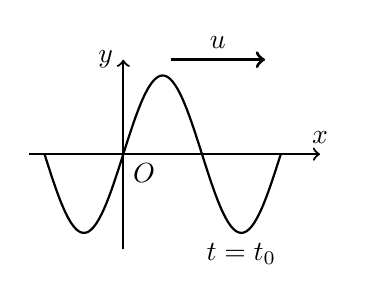
\begin{tikzpicture}
    \draw [thick,->] (-1.2,0)--(2.5,0) node [anchor=south] {$x$};
    \draw [thick,->] (0,-1.2)--(0,1.2) node [anchor=east] at (0,1.2) {$y$};
    \draw [thick] (-1,0) sin (-0.5,-1) cos (0,0) sin (0.5,1) cos (1,0) sin (1.5,-1) node [anchor=north] {$t=t_0$} cos (2,0);
    \node [anchor=north west] at (0,0) {$O$};
    \draw [very thick,->] (0.6,1.2)--(1.8,1.2) node [anchor=south,midway] {$u$};
\end{tikzpicture}
\vfill
\end{paracol}
\begin{solution}*
    由图可知，$t=t_0$时刻原点处的质点$v<0$，所以此时的相位为$\varphi_0=\pi/2$.\sokka{B}
\end{solution}

\begin{choice}{D}[双缝干涉]
    在双缝干涉实验中，光的波长为$500\mathrm{nm}$，双缝间距为$2\mathrm{mm}$，双缝与屏的间距为$400\mathrm{cm}$. 则干涉图样的明纹间距为
    \begin{tasks}(4)
        \task $0.9\mathrm{mm}$
        \task $0.5\mathrm{mm}$
        \task $1.2\mathrm{mm}$
        \task $1.0\mathrm{mm}$
    \end{tasks}
\end{choice}
\begin{solution}*
    条纹间距$\Delta x=\lambda D/d=1\mathrm{mm}$.\sokka{D}
\end{solution}

\begin{choice}{C}[平面简谐波的物理量]
    在下面几种说中，正确的是
    \begin{tasks}(2)
        \task 波源不动时，波源的振动、波动周期在数值上不同
        \task 波源振动的速度与波速相同
        \task! 在波传播方向上的任一质点的振动相位总是比波源的相位滞后（按差值不大于$\pi$计）
        \task! 在波传播方向上的任一质点的振动相位总是比波源的相位超前（按差值不大于$\pi$计）
    \end{tasks}
\end{choice}
\begin{solution}
    \begin{itemize}
        \item 波速是波在介质中的传播速度，波源的振动速度是质点在某一刻的瞬时速度，所以B选项错误.
        \item 各质点在波源的带动下做受迫振动，二者周期相等，所以A选项错误；由$\Delta\varphi=\frac{2\pi\delta}{\lambda}$可知D选项错误.
    \end{itemize}
\end{solution}

\begin{paracol}{2}
    \begin{choice}{D}[光程和光程差]
        如图所示，$S_1,\ S_2$为两相干波源，其振幅均为$0.5\mathrm{m}$，频率均为$100\mathrm{Hz}$.但当$S_1$为波峰时，$S_2$为波谷.设在媒质中的波速为$10\mathrm{m/s}$，则两波抵达$P$点时的相位差和$P$点的合振幅为
        \begin{tasks}(4)
            \task $200\pi,\ 0\mathrm{m}$
            \task $200\pi,\ 0.5\mathrm{m}$
            \task $201\pi,\ 0.5\mathrm{m}$
            \task $201\pi,\ 0\mathrm{m}$
        \end{tasks}    
    \end{choice}
\switchcolumn\centering
\vfill
\begin{tikzpicture}
    \draw [thick] (0,3)--(0,0)--(4,0) ;
    \shade [ball color=H1] (0,0) circle (0.1) node [anchor=east] {$S_1$};
    \shade [ball color=H1] (4,0) circle (0.1) node [anchor=west] {$S_2$};
    \shade [ball color=H1] (0,3) circle (0.1) node [anchor=south] {$P$};
    \length{(0.375,3)}{(0.375,0)}{$15\mathrm{m}$}{(0,-0.5)}
    \length{(0,-0.25)}{(4,-0.25)}{$20\mathrm{m}$}{(0.75,0)}
\end{tikzpicture}
\vfill
\end{paracol}
\begin{solution}
    相干波的波长为$\lambda=u/f=10\mathrm{cm}$.由题意得$S_2$与$S_1$在波源处相位差为$\pi$.所以到$P$点时的相差为
    $$\Delta\varphi=\varphi_2-\varphi_1-\frac{2\pi}{\lambda}\ab(\overline{S_2P}-\overline{S_1P})=201\pi$$
    所以$P$点的合振幅为$A=\sqrt{A_1^2+A_2^2+2A_1A_2\cos{\Delta\varphi}}=0\mathrm{m}$.
\end{solution}

\begin{choice}{A}[光程和光程差]
    $S_1,\ S_2$是两个相干光源，它们到$P$点的距离分别为$r_1$和$r_2$.路径$S_1P$垂直穿过一块厚度为$t_1$，折射率为$n_1$的介质板，路径$S_2P$垂直穿过厚度为$t_2$，折射率为$n_2$的另一介质板，其余部分可看作真空，这两条路径的光程差等于
    \begin{tasks}(2)
        \task $\ab[r_2+\ab(n_2-1)t_2]-\ab[r_1+\ab(n_1-1)t_1]$
        \task $\ab(r_2+n_2t_2)-\ab(r_1+n_1t_1)$
        \task $\ab(r_2-n_2t_2)-\ab(r_1-n_1t_1)$
        \task $\ab[r_2+\ab(n_2+1)t_2]-\ab[r_1+\ab(n_1+1)t_1]$
    \end{tasks}
\end{choice}
\begin{solution}*
    两路径的光程分别为$r_{1,2}+\ab(n_{1,2}-1)t_{1,2}$.\sokka{A}
\end{solution}

\begin{choice}{A}[牛顿环]
    用单色光垂直照射在观察牛顿环的装置上，当平凸透镜垂直向上缓慢平移而远离平面玻璃时，可以观察到这些环状干涉条纹
    \begin{tasks}(4)
        \task 向中心收缩
        \task 向外扩张
        \task 向右平移
        \task 向左平移
    \end{tasks}
\end{choice}
\begin{solution}*
    向中心收缩光程差减小，可抵消透镜上移时导致的光程差增大.\sokka{A}
\end{solution}

\begin{paracol}{2}
    \begin{choice}{B}[劈尖干涉]
        如图所示，两个直径有微小差别的彼此平行的滚柱之间的距离为$L$，夹在两块平板透光晶体的中间，形成空气劈尖.当单色光垂直入射时，产生等厚干涉条纹，如果两滚柱之间的距离$L$变小，则在$L$范围内干涉条纹的
        \begin{tasks}(2)
            \task 数目不变，间距变大
            \task 数目不变，间距变小
            \task 数目增加，间距变小
            \task 数目减少，间距变大
        \end{tasks}
    \end{choice}
    \switchcolumn\centering
    \vfill
    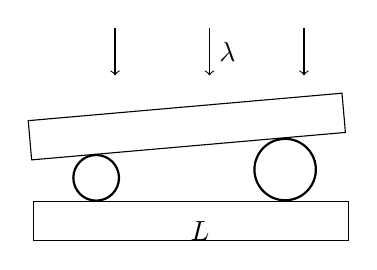
\begin{tikzpicture}
        \draw (-2,0) rectangle (2,0.5);
        \draw [rotate=5,xshift=0.78mm] (-2,1.2) rectangle (2,1.7);
        \draw [thick] (-1.2,0.8) circle (0.29);
        \draw [thick] (1.2,0.905) circle (0.39);
        \length{(-1.2,0.25)}{(1.2,0.25)}{$L$}{(0.25,0)}
        \foreach \a in {-1.2,0,1.2}
        \draw [->,xshift=\a cm] (0,2.7)--(0,2.1);
        \node [anchor=west] at (0,2.4) {$\lambda$};
    \end{tikzpicture}
    \vfill
\end{paracol}
\begin{solution}*
    两滚筒间距变小相当于劈尖的顶角在变大，根据条纹间距公式$\Delta x=\frac{\lambda}{2\theta}$所以条纹间隔变小；对于某条纹路，其光程差是确定的，所以数目不变.\sokka{B}
\end{solution}

\begin{choice}{D}[弗琅禾费衍射]
    在单缝夫琅和费衍射实验中，波长为$\lambda$的单色光垂直入射在宽度为$a=5\lambda$的单缝上，对应于衍射角为$30^{\circ}$的方向，单缝处波阵面可分成的半波带数目为
    \begin{tasks}(4)
        \task 6个
        \task 4个
        \task 7个
        \task 5个
    \end{tasks}
\end{choice}
\begin{solution}*
    由衍射公式$a\sin{\theta}=k\lambda$得$k=5/2$，可分成的半波带数目为$2k=5$.\sokka{D}
\end{solution}

\section{填空题（共25分）}
{
\begin{paracol}{2}
\begin{problem}[单摆][5]
    在$t=0$时，振幅为$A$，周期为$T$的单摆分别处于图示的三种状态.若选单摆的平衡位置为坐标原点，坐标指向正右方，则单摆做小角度摆动的振动表达式（用余弦函数表示）分别为(a)\ans{$x=A\cos\ab(\frac{2\pi}{T}t-\frac{\pi}{2})$}，(b)\ans{$x=A\cos\ab(\frac{2\pi}{T}t+\frac{\pi}{2})$}，(c)\ans{$x=A\cos{\ab(\frac{2\pi}{T}t+\pi)}$}
\end{problem}
\switchcolumn\centering
\vfill
\begin{tikzpicture}
    \foreach \a in{0,2,4}
    \draw [thick,xshift=\a cm] (-0.8,0)--(0.8,0);
    \foreach \b in{0,2,4}
    \fill [pattern color=normalcolor,pattern=north east lines,xshift=\b cm] (-0.75,0) rectangle (0.75,0.2);
    \draw [thick] (0,0)--(0,-3);
    \draw [->] (0.1,-3)--(0.7,-3) node [anchor=south] {$v_0$};
    \shade [ball color=H1] (0,-3) circle (0.1);

    \draw [thick] (2,0)--(2,-3);
    \draw [->] (1.9,-3)--(1.3,-3) node [anchor=south] {$v_0$};
    \shade [ball color=H1] (2,-3) circle (0.1);

    \draw [thick,dashed] (4,0)--(4,-3);
    \draw [thick] (4,0)--(2.8,-2.75) node [anchor=north] {$v_0=0$};
    \shade [ball color=H1] (2.8,-2.75) circle (0.1);

    \node [anchor=north] at (0,-3.2) {(a)};
    \node [anchor=north] at (2,-3.2) {(b)};
    \node [anchor=north] at (4,-3.2) {(c)};
\end{tikzpicture}
\vfill
\end{paracol}
\begin{solution}*
    三种情况的状态和对应的相位分别为$x=0,\ v>0,\ \varphi=-\frac{\pi}{2}$；$x=0,\ v<0,\ \varphi=\frac{\pi}{2}$；$x=-A,\ v=0,\ \varphi=\pi$.所以振动表达式分别为$A\cos\ab(\frac{2\pi}{T}t-\frac{\pi}{2}),\ A\cos\ab(\frac{2\pi}{T}t+\frac{\pi}{2}),\ A\cos{\ab(\frac{2\pi}{T}t+\pi)}$.
\end{solution}

\begin{problem}[弹簧振子][4]
    一物块悬挂在弹簧下方做简谐振动，当这物块的位移等于振幅的一半时，其动能是总能量的\ans{$\frac{3}{4}$}（设平衡位置处势能为零）.当这物块在平衡位置时，弹簧的长度比原长长$\Delta l$，这一振动系统的周期为\ans{$2\pi\sqrt{\Delta l/g}$}.
\end{problem}
\begin{solution}*
    此时物块动能为$E_k=\frac{1}{2}kA^2-\frac{1}{2}k\ab(\frac{A}{2})^2=\frac{3}{8}kA^2$，所以此时物块动能是总能量的$\frac{\frac{3}{8}kA^2}{\frac{1}{2}kA^2}=\frac{3}{4}$；弹簧的劲度系数$k=mg/\Delta l$，由弹簧振子周期表达式得系统的周期为$T=2\pi\sqrt{m/k}=2\pi\sqrt{\Delta l/g}$.
\end{solution}

\begin{paracol}{2}
    \begin{problem}[平面简谐波的波函数][3]
        右图所示为一平面简谐波在$t=2\mathrm{s}$时的波形图，则$O$点的振动方程为$y_o=$\ans{$0.04\cos{\ab(0.4\pi t-1.3\pi)}$}.
    \end{problem}
    \begin{solution}*
    由图可知简谐波的振幅$A=0.04\mathrm{m}$；波长$\lambda=0.4\mathrm{m}$，所以其角频率$\omega=\frac{2\pi u}{\lambda}=0.4\pi\mathrm{s}^{-1}$.在此刻$O$点处的质点$v>0$，所以此时的相位$\varphi_0=-\frac{\pi}{2}$，$t=0$时刻$O$点的相位$\varphi=-0.4\pi \cdot 2-\frac{\pi}{2}=-1.3\pi$，$O$点的振动方程$y_o=0.04\cos{\ab(0.4\pi t-1.3\pi)}$.
    \end{solution}
    \switchcolumn\centering
    \vfill
    \begin{tikzpicture}[decoration={markings,
        mark=between positions 0.05 and 1 step 6mm
        with {\draw [-,gray] (0,-0.1) -- (0,0.1);}}]
        \draw [thick,->,postaction=decorate] (-0.2,0)--(4.2,0) node [anchor=south] {$x/\mathrm{m}$};
        \draw [thick,->] (0,-1.2)--(0,1.5) node [anchor=south] {$y/\mathrm{m}$};
        \node [anchor=north east] at (0,0) {$O$};
        \draw [thick] (0,0) sin (0.6,-1) cos (1.2,0) sin (1.8,1) cos (2.4,0) sin (3,-1) cos (3.6,0);
        \draw [very thick,->] (2,1.2)--(3.2,1.2) node [anchor=south,midway] {$u=0.08\mathrm{m/s}$};
        \node [anchor=north] at (0.6,0) {$0.1$} node [anchor=north] at (1.8,0) {$0.3$} node [anchor=north] at (3,0) {$0.5$};
        \draw [dashed] (0,1)--(1.8,1) node [anchor=east,at start] {$0.04$};
    \end{tikzpicture}
    \vfill
\end{paracol}

\begin{problem}[多普勒效应][3]
    一静止的报警器，其频率为$1000\mathrm{Hz}$.有一汽车以$79.2\mathrm{km}$的时速远离报警器时，坐在汽车里的人听到的报警声的频率是\ans{$935.3\mathrm{Hz}$}（设空气中声速为$340\mathrm{m/s}$）.
\end{problem}
\begin{solution}
    已知多普勒效应观察者（Observer）和发射源（Source）的的频率关系为
    $$\nu=\frac{u\pm v_o}{u\mp v_s}\nu_0$$
    
    $v_o$为观察者速度，接近为$+$，远离为$-$；$v_s$为发射源速度，接近为$-$，远离为$+$.观察者远离，其所听频率为
    $$\nu=\frac{340-22}{340}\times 550\mathrm{Hz}\approx 935.3\mathrm{Hz}$$
\end{solution}

\begin{problem}[光的相干条件][4]
    在双缝干涉实验中，用白光照射时，明纹会出现彩色条纹，明纹外侧呈\ans{红}颜色；如果用纯绿色滤光片和纯蓝色滤光片分别盖住两缝，则\ans{不能}产生干涉条纹（填能或不能）.
\end{problem}
\begin{solution}*
    波长越大，明纹张角越大，所以外侧呈红色；根据干涉条件「频率相等」，此时不能产生干涉条纹.
\end{solution}

\begin{problem}[劈尖干涉][3]
    用波长为$\lambda$的单色光垂直照射劈尖膜（$n_1>n_2>n_3$），观察反射光干涉.从劈尖顶开始算起，第二条暗纹中心所对应的膜厚度为\ans{$3\lambda/4n_2$}.
\end{problem}
\begin{solution}*
    由暗纹条件$\delta=2n_2h=\frac{2k-1}{2}\lambda$得$k=2$时，$h=\frac{3\lambda}{4n_2}$.
\end{solution}

\begin{problem}[弗琅禾费衍射][3]
    单缝弗琅禾费衍射的第一级暗纹发生在衍射角$30^{\circ}$的方向上，所用单色光波长$\lambda=600\mathrm{nm}$，则单缝宽度为\ans{$1.2\mu\mathrm{m}$}.
\end{problem}
\begin{solution}*
    由暗纹条件$a\sin{\varphi}=k\lambda$，代入$k=1,\ \varphi=30^{\circ}$得$a=2\lambda=1.2\mu\mathrm{m}$.
\end{solution}
}

\section{计算题（共48分）}
{
\begin{problem}[简谐振动][10]
    一质点按如下规律沿$x$轴做简谐振动$x=0.2\cos{\ab(4\pi t+\frac{1}{3}\pi)}\ \mathrm{(SI)}$，求此振动的周期、振幅、初相、速度最大值和加速度最大值.
\end{problem}
\begin{solution}
\begin{multicols}{2}
    \begin{itemize}
        \item 周期：$T=2\pi/\omega=0.5\mathrm{s}$\point{2}
        \item 振幅：$A=0.2\mathrm{m}$\point{2}
        \item 初相：$\varphi_0=\frac{1}{3}\pi$\point{2}
        \item 速度最大值：$v_{\max}=\omega A=0.8\pi\mathrm{m/s}$\point{2}
        \item 加速度最大值：$a_{\max}=\omega^2 A=3.2\pi^2\mathrm{m/s}^2$\point{2}
    \end{itemize}
\end{multicols}
\end{solution}

\begin{problem}[简谐振动，平面简谐波的波函数][8]
    某质点做简谐振动，周期为$2\mathrm{s}$，振幅为$0.06\mathrm{m}$，$t=0$时刻，质点恰好处在平衡位置并向负方向运动，求
    \begin{enumerate}
        \item 该质点的振动方程.
        \item 此振动以速度$u=3\mathrm{m/s}$沿$x$轴正方向传播时，形成的一维简谐波的波动方程（以平衡位置为坐标原点）.
        \item 该波的波长.
    \end{enumerate}
\end{problem}
\begin{solution}
    \begin{enumerate}
        \item 由题意得，质点的角频率$\omega=\frac{2\pi}{T}=1\pi\mathrm{s}^{-1}$，质点的初相$\varphi=\frac{\pi}{2}$.故质点的振动方程为
        \[y_0=0.06\cos{\ab(\pi t+\frac{\pi}{2})}\eqno\point{2}\]
        \item 波动表达式$y=A\cos{\ab[\omega\ab(t-\frac{x}{u})+\varphi]}=0.06\cos{\ab[\pi\ab(t-\frac{x}{3})+\frac{\pi}{2}]}$.\point{3}
        \item 波长$\lambda=uT=6\mathrm{m}$.\point{2}
    \end{enumerate}
\end{solution}

\begin{problem}[双缝干涉][6]
    用一束$\lambda=580\mathrm{nm}$激光垂直照射一双缝，在缝后$2.0\mathrm{m}$处的墙上观察到中央明纹和第一级明纹的间隔为$15\mathrm{cm}$.求
    \begin{enumerate}
        \item 两缝的间距.
        \item 在中央明纹以上还能看到几条明纹.
    \end{enumerate}
\end{problem}
\begin{solution}
    \begin{enumerate}
        \item 由$\Delta x=\lambda D/d$得两缝的间距$d=\lambda D/\Delta x=7.73\mu\mathrm{m}$.\point{3}
        \item 由明纹条件$d\sin{\theta}=k\lambda$，取$\theta$最大值为$90^{\circ}$，中央明纹以上能看到的明纹条数为$k=\left\lfloor d/\lambda\right\rfloor=13$.\point{3}
    \end{enumerate}
\end{solution}

\begin{problem}[驻波][10]
    入射波的表达式为$y_1=A\cos{\ab[2\pi\ab(\frac{t}{T}+\frac{x}{\lambda})]}$，在$x=0$发生反射，反射点为一固定端，设反射时无能量损失.求
    \begin{enumerate}
        \item 反射波的表达式
        \item 驻波的表达式
        \item 波腹、波节的位置
    \end{enumerate}
\end{problem}
\begin{solution}
\begin{enumerate}
    \item 到达反射端后，波的传播方向发生变化，同时因半波损失带有$\pi$的相位差.所以反射波的表达式为\point{1}
    $$y_2=A\cos{\ab[2\pi\ab(\frac{t}{T}-\frac{x}{\lambda})+\pi]}\eqno\point{2}$$
    \item 驻波表达式$y=y_1+y_2=2A\cos{\ab(\frac{2\pi t}{T}+\frac\pi2)}\cos{\ab(\frac{2\pi x}{\lambda}-\frac{\pi}{2})}$.\point{3}
    \item 
    波腹的位置$\cos{\ab(\frac{2\pi x}{\lambda}-\frac{\pi}{2})}=\pm 1,\ x=\frac{2k+1}{4}\lambda,\ k=0,1,2,\cdots$；\point{2}

    波节的位置$\cos{\ab(\frac{2\pi x}{\lambda}-\frac{\pi}{2})}=0,\ x=\frac{k}{2}\lambda,\ k=0,1,2,\cdots$.\point{2}
\end{enumerate}
\end{solution}

\begin{problem}[劈尖干涉][8]
    用波长$500\mathrm{nm}$的单色光垂直照射到由两块光学平玻璃构成的空气劈形膜上.在观察反射光的干涉现象中，距劈形膜棱边$l=1.56\mathrm{cm}$的$A$处是从棱边算起的第四条暗纹中心.
    \begin{enumerate}
        \item 求此空气劈形膜的劈尖角$\theta$.
        \item 改用$600\mathrm{nm}$的单色光垂直照射到此劈尖上仍观察反射光的干涉条纹，$A$处是明条纹还是暗条纹？
        \item 在第2问的情形从棱边到$A$处的范围共有几条明纹，几条暗纹？
    \end{enumerate}
\end{problem}
\begin{solution}
    \begin{enumerate}
        \item 考虑半波反射，两束光的光程差为$\delta=2h_k+\frac{\lambda}{2}$，由暗纹条件
        \[2h_4+\frac{\lambda}{2}=\frac{2k-1}{2}\lambda=\frac{2\times 4-1}{2}\lambda\]
        利用小角度近似得劈尖角$\theta\approx\frac{h_4}{l}=4.81\times 10^{-5}\mathrm{rad},\ h_4=750\mathrm{nm}$.
        \item 此时光程差$\delta=2h_4+\frac{\lambda^{\prime}}{2}=1800\mathrm{nm}=3\lambda^{\prime}$，满足明纹条件$\delta=k\lambda$. 所以$A$处是第3条明纹.
        \item 由棱边处的光程差$\delta=\frac{\lambda}{2}$可知棱边处为暗纹.所以共有$3$条明纹，$3$条暗纹.
    \end{enumerate}
\end{solution}

\begin{problem}[弗琅禾费衍射][6]
    今有白光形成单缝弗琅禾费衍射，若其中某一光波的第四级明纹和红光（$\lambda=600\mathrm{nm}$）的第三级明纹相重合，求这一光波的波长.
\end{problem}
\begin{solution}*
    明纹位置$a\sin{\varphi}=\pm\frac{2k+1}{2}\lambda$，由重合条件$\frac{2\times 3+1}{2}\lambda=\frac{2\times 4+1}{2}\lambda^{\prime}$得光波波长$\lambda^{\prime}=\frac{7}{9}\lambda=446.7\mathrm{nm}$.
\end{solution}
}